\section{Requisiti}\label{Requisiti}

Il team \texttt{Agents of S.W.E.} ha classififcato e assegnato i requisiti con un identificativo univoco, secondo quanto definito nel documento \textit{Norme di progetto v2.0.0} nella sezione §2.2.2.1.

\subsection{Requisiti Funzionali}\label{RF}
\begin{center}
\begin{longtable}[c]{|m{.13\textwidth}|m{.47\textwidth}|m{.2\textwidth}|m{.11\textwidth}|}
\hline
\rowcolor{bluelogo}\textbf{\textcolor{white}{ID}} & \textbf{\textcolor{white}{Descrizione}} & \textbf{\textcolor{white}{Obbligatorietà}} & \textbf{\textcolor{white}{Fonti}}\\
\hline \hline
\endhead
ROF1 & L'utente deve poter aggiungere una rete bayesiana al sistema & Obbligatorio & UC1\\
\hline
\rowcolor{grigio}ROF1.1 & Il Sistema deve mettere a disposizione un pulsante per avviare l'operazione di selezione del file, contenente la definizione della rete, da caricare & Obbligatorio & UC1\\
\hline
ROF1.2 & Il Sistema deve consentire all'utente di selezionare un file da caricare & Obbligatorio & UC1\\
\hline
\rowcolor{grigio}ROF1.3 & Il Sistema deve mettere a disposizione dell'utente un bottone per avviare l'operazione di caricamento & Obbligatorio & UC1\\
\hline
ROF1.4 & Il Sistema deve visualizzare un messaggio di errore nel caso l'operazione di caricamento del file non sia andata a buon fine & Obbligatorio & UC1 UC8\\
\hline
\rowcolor{grigio}ROF1.4.1 & Il Sistema deve controllare l'estensione del file caricato, accettando come input solamente file in formato \textit{.JSON} & Opzionale & UC1 UC8\\
\hline
RFF1.4.2 & Il Sistema deve visualizzare un messaggio di errore nel caso in cui la struttura interna del file selezionato sia errata & Opzionale & UC1 UC8\\
\hline
\rowcolor{grigio}ROF1.5 & Il Sistema deve interpretare il file caricato, al fine di costruire la rete bayesiana attraverso la sua definizione & Obbligatorio & UC1\\
\hline
RDF1.6 & Il Sistema deve mantenere in memoria, in caso di riavvio, l'ultima rete bayesiana caricata dall'utente & Desiderabile & Decisione Interna\\
\hline
\rowcolor{grigio}ROF2 & L'utente deve poter collegare un flusso di dati ad ogni nodo desiderato della rete preesistente & Obbligatorio & UC2\\
\hline
ROF2.1 & Il Sistema deve interpretare la rete bayesiana caricata, al fine di estrapolarne i nodi e fornirli all'utente sotto forma di lista & Obbligatorio & 16\\
\hline
\rowcolor{grigio}ROF2.1.1 & Il Sistema deve mostrare, per ogni nodo, il nominativo dello stesso & Obbligatorio & UC16\\
\hline
ROF2.1.2 & Il Sistema deve mostrare, per ogni nodo, una corrispondente checkbox che identifichi lo stato dello stesso: collegato ad un flusso dati oppure no & Obbligatorio & UC16 UC2\\
\hline
\rowcolor{grigio}ROF2.5 & Il Sistema deve mettere a disposizione dell'utente le impostazioni necessarie per effettuare correttamente il collegamento desiderato & Obbligatorio & UC2\\
\hline
ROF2.5.3 & Il Sistema deve fornire un elenco dei flussi dati disponibili contestualmente alla sorgente di dati selezionata & Obbligatorio & UC2.3\\
\hline
\rowcolor{grigio}ROF2.5.4 & L'utente deve poter selezionare il flusso dati desiderato per il collegamento & Obbligatorio & UC2.3\\
\hline
ROF2.5.5 & Il Sistema deve mostrare la lista dei possibili stati del nodo selezionato & Obbligatorio & UC2.3\\
\hline
\rowcolor{grigio}ROF2.5.6 & Il Sistema deve mettere a disposizione dell'utente, per ogni stato del nodo, i campi dati necessari alla definizione di un livello di soglia connesso al flusso dati selezionato & Obbligatorio & UC2.3\\
\hline
ROF2.5.6.1 & Il Sistema deve mettere a dispozione dell'utente un campo dati che permetta di definire il valore numerico della soglia & Obbligatorio & UC2.3\\
\hline
\rowcolor{grigio}ROF2.5.6.2 & Il Sistema deve mettere a dispozione dell'utente un campo dati che permetta di definire se il valore numerico definito per la soglia sia un minimo oppure un massimo & Obbligatorio & UC2.3\\
\hline
RDF2.5.6.3 & Il Sistema deve mettere a dispozione dell'utente un campo dati che permetta di definire se la soglia sia critica oppure no & Desiderabile & UC2.3 VER-2019-02-08\\
\hline
\rowcolor{grigio}ROF2.5.7 & L'utente deve poter editare i campi dati per definire correttamente un livello di soglia al di sotto, o al di sopra del quale la probabilità associata a quel dato stato risulta pari al 100\%, mentre le probabilità associate agli altri stati risultano pari allo 0\% & Obbligatorio & UC2.3\\
\hline
ROF2.5.8 & Il Sistema deve mettere a disposizione dell'utente un bottone per confermare le scelte riguardardanti la definizione della soglia & Obbligatorio & UC2.3\\
\hline
\rowcolor{grigio}ROF2.5.9 & Il Sistema deve visualizzare un messaggio di errore nel caso in cui l'utente abbia confermato le proprie scelte riguardanti il collegamento del singolo nodo in esame, senza aver correttamente definito il livello di soglia & Obbligatorio & UC2.3 UC14\\
\hline
ROF2.5.10 & Il Sistema deve aggiornare la lista di checkbox, registrando il nuovo stato di ogni nodo (collegato o meno ad un flusso dati) & Obbligatorio & UC2\\
\hline
ROF3 & L'utente deve poter impostare una politica temporale per il ricalcolo delle probabilità condizionate associate ai nodi della rete bayesiana & Obbligatorio & UC3\\
\hline
\rowcolor{grigio}ROF3.3 & L'utente deve avere la possibilità di definire una politica temporale & Obbligatorio & UC3\\ 
\hline
ROF3.3.1 & Il Sistema deve mettere a disposizione un pulsante per accedere al pannello di configurazione di una politica temporale & Obbligatorio & UC3\\
\hline
\rowcolor{grigio}ROF3.3.2 & Il Sistema deve mettere a disposizione dell'utente un pannello di configurazione contenente i campi dati necessari alla definizione di una politica temporale & Obbligatorio & UC3\\
\hline
ROF3.3.2.1 & Il Sistema deve mettere a dispozione dell'utente un campo dati che permetta di definire il valore numerico del timeout ciclico & Obbligatorio & UC3\\
\hline
\rowcolor{grigio}ROF3.3.2.2 & Il Sistema deve mettere a dispozione dell'utente un campo dati che permetta di definire l'unità di misura temporale associata al timeout & Obbligatorio & UC3\\
\hline
ROF3.3.3 & L'utente deve poter editare i campi dati per definire correttamente la politica temporale desiderata & Obbligatorio & UC3\\
\hline
\rowcolor{grigio}ROF3.4 & Il Sistema deve mettere a disposizione dell'utente un bottone per confermare la politica temporale da lui definita & Obbligatorio & UC3\\
\hline
ROF3.5 & Il Sistema deve visualizzare un messaggio di errore nel caso in cui l'utente abbia confermato una politica temporale non correttamente definita & Obbligatorio & UC3 UC15\\
\hline
\rowcolor{grigio}ROF4 & Il Sistema deve fornire i dati relativi ai nodi della rete bayesiana non collegati al flusso & Obbligatorio & UC4 UC20\\
\hline
ROF4.4 & Il Sistema deve mettere a disposizione dell'utente un pulsante per avviare il monitoraggio dei dati & Obbligatorio & UC20\\
\hline
\rowcolor{grigio}ROF4.4.3 & Il Sistema deve visualizzare un messaggio di errore nel caso in cui l'utente abbia avviato il monitoraggio senza aver preventivamente impostato la politica temporale per il ricalcolo delle probabilità & Obbligatorio & UC20 UC12\\
\hline
ROF4.4.4 & Il Sistema deve visualizzare un messaggio di errore nel caso in cui l'utente abbia avviato il monitoraggio senza aver preventivamente collegato almeno un nodo della rete bayesiana al flusso dati & Obbligatorio & UC20 UC9\\
\hline
ROF4.5 & Il Sistema deve fornire all'utente una lista di probabilità dinamiche associate ai nodi della rete & Obbligatorio & UC4\\
\hline
\rowcolor{grigio}ROF4.6 & Il Sistema deve aggiornare periodicamente le probabilità in base a quanto definito come policy per il ricalcolo delle probabilità & Obbligatorio & UC4\\
\hline
RDF4.6.1 & Il Sistema, indipendentemente dalla politica temporale stabilita dall'utente, deve ricalcolare le probabilità al verificarsi del superamento di una soglia critica associata ad uno stato di un nodo collegato al flusso di monitoraggio & Desiderabile & UC4 VER-2019-02-08\\
\hline
\rowcolor{grigio}RFF5 & L'utente deve poter definire alert basati sui dati relativi ai nodi della rete bayesiana non collegati al flusso & Opzionale & Capitolato\\
\hline
RFF5.1 & Il Sistema deve mettere a disposizione di \textit{Grafana}, i dati per l'operazione di creazione di alert ad essi associati da parte dell'utente & Opzionale & Capitolato UC4\\
\hline
\rowcolor{grigio}RFF6.1 & Il Sistema deve mettere periodicamente a disposizione della piattaforma \textit{Grafana}, i dati aggiornati per il monitoraggio costante dello stato degli alert & Opzionale & UC4\\
\hline
\caption{Requisiti Funzionali}
\end{longtable}
\end{center}


%\subsection{Requisiti Prestazionali}\label{RP}
\subsection{Requisiti di Qualità}\label{RQ}
\begin{center}
\begin{longtable}[c]{|m{.09\textwidth}|m{.48\textwidth}|m{.2\textwidth}|m{.12\textwidth}|}
\hline
\rowcolor{bluelogo}\textbf{\textcolor{white}{ID}} & \textbf{\textcolor{white}{Descrizione}} & \textbf{\textcolor{white}{Obbligatorietà}} & \textbf{\textcolor{white}{Fonti}}\\
\hline \hline
\endhead
ROQ1 & È necessario fornire un manuale utente, per l'utilizzo del prodotto, in formato \textit{pdf} & Obbligatorio & Capitolato\\
\hline
\rowcolor{grigio}ROQ1.1 & Il manuale utente deve essere disponibile in lingua italiana & Obbligatorio & Decisione Interna\\
\hline
RDQ1.2 & Il manuale utente deve essere disponibile in lingua inglese & Desiderabile & Decisione Interna\\
\hline
\rowcolor{grigio}ROQ2 & È necessario fornire un manuale per la manutenzione ed estensione del prodotto & Obbligatorio & Capitolato\\
\hline
ROQ2.1 & Il manuale di manutenzione/estensione deve essere disponibile in lingua italiana & Obbligatorio & Decisione Interna\\
\hline
\rowcolor{grigio}RDQ2.2 & Il manuale di manutenzione/estensione deve essere disponibile in lingua inglese & Desiderabile & Decisione Interna\\
\hline
ROQ3 & Il prodotto deve essere sviluppato in modo concorde a quanto stabilito nelle \textit{Norme di Progetto v2.0.0} & Obbligatorio & Decisione Interna\\
\hline
\rowcolor{grigio}RDQ5 & Il codice sorgente del plug-in deve essere reperibile in una repository pubblica su \textit{GitHub}\glossario o su altre piattaforme di condivisione & Desiderabile & Capitolato \\
\hline
RDQ6 & Il plug-in deve essere pubblicato nella sezione plug-in di \textit{Grafana}, disponibile all'indirizzo \url{https://grafana.com/plugins}   & Desiderabile & Decisione Interna \\
\hline
\rowcolor{grigio}RDQ7 & Il plug-in deve essere compatibile con la versione 6.0.0 di \textit{Grafana}, pubblicata in data 2019-02-25  & Desiderabile & Decisione Interna\\
\hline
RDQ8 & La struttura della directory del plug-in deve essere conforme con quanto indicato dalla documentazione di \textit{Grafana}, al link: \url{http://docs.grafana.org/plugins/developing/plugin-review-guidelines/}  & Desiderabile & Decisione Interna \\
\hline
\caption{Requisiti di Qualità}
\end{longtable}
\end{center}

\pagebreak

\subsection{Requisiti di Vincolo}\label{RV}
\begin{center}
\begin{longtable}[c]{|m{.1\textwidth}|m{.53\textwidth}|m{.25\textwidth}|}
\hline
\rowcolor{bluelogo}\textbf{\textcolor{white}{ID}} & \textbf{\textcolor{white}{Descrizione}} & \textbf{\textcolor{white}{Fonti}}\\
\hline \hline
\endhead
ROV1 & Il plug-in deve essere sviluppato in linguaggio \textit{ECMAScript6} & \textit{Grafana}: guida per gli sviluppatori.\\
\hline
\rowcolor{grigio}ROV2 & Il punto di ingresso per il plug-in deve essere sviluppato nel file "module.js" & \textit{Grafana}: guida per gli sviluppatori\\
\hline
ROV3 & Va utilizzato un qualsiasi build system\glossario che supporti \textit{systemjs}\glossario & \textit{Grafana}: guida per gli sviluppatori\\
\hline
\rowcolor{grigio}ROV4 & Il codice sorgente del plug-in deve essere open source & Capitolato\\
\hline
ROV5 & La rete bayesiana è definita in un file formato \textit{.JSON} & Capitolato\\
\hline
\rowcolor{grigio}ROV6 & L'interfaccia grafica del plug-in è sviluppata utilizzando \textit{HTML5}\glossario, \textit{CSS3}\glossario e \textit{Angularjs}\glossario & \textit{Grafana}: guida per gli sviluppatori \\
\hline
ROV8 & Il Sistema deve funzionare sul browser \textit{Chrome} dalla versione 58 & \hyperref[SupportoECMAScript]{Supporto al linguaggio ECMAScript6 (§\ref*{SupportoECMAScript})}\\
\hline
\rowcolor{grigio}ROV9 & Il Sistema deve funzionare sul browser \textit{Microsoft Edge} dalla versione 14 & \hyperref[SupportoECMAScript]{Supporto al linguaggio ECMAScript6 (§\ref*{SupportoECMAScript})}\\
\hline
ROV10 & Il Sistema deve funzionare sul browser \textit{Firefox} dalla versione 54 & \hyperref[SupportoECMAScript]{Supporto al linguaggio ECMAScript6 (§\ref*{SupportoECMAScript})}\\
\hline
\rowcolor{grigio}ROV11 & Il Sistema deve funzionare sul browser \textit{Safari} dalla versione 10 & \hyperref[SupportoECMAScript]{Supporto al linguaggio ECMAScript6 (§\ref*{SupportoECMAScript})}\\
\hline
ROV12 & Il plug-in deve funzionare per l'ultima versione di \textit{Grafana} disponibile in tempo di ingresso ad RR: v5.4.3 & Decisione Interna\\
\hline
\caption{Requisiti di Vincolo}
\end{longtable}
\end{center}

\begin{figure}[H]
	\begin{center}
		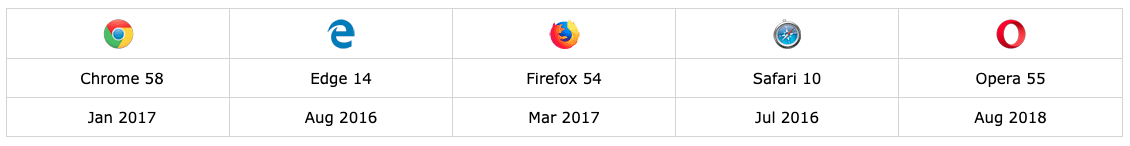
\includegraphics[scale=0.4]{./images/ES6_Support.png}
		 \caption{Supporto al Linguaggio ECMAScript6. Immagine da: \url{https://www.w3schools.com/js/js_es6.asp}}
		 \label{SupportoECMAScript}	
	\end{center}
\end{figure}

\pagebreak

%\footnote{Il supporto al linguaggio ECMASCript 6 è il seguente:\\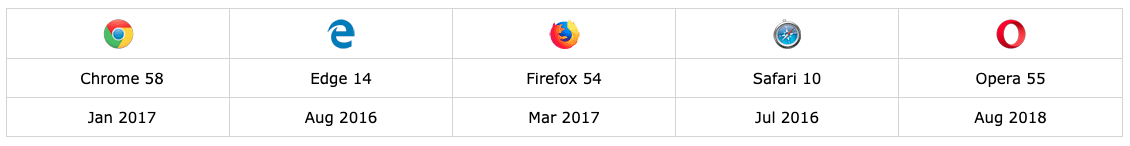
\includegraphics[scale=0.3]{./images/ES6_Support.png}\\Immagine da: \url{https://www.w3schools.com/js/js_es6.asp}} 

\subsection{Tacciamento Fonti-Requisiti}\label{Tracciamento}
\begin{center}
\begin{longtable}[c]{|c|m{.15\textwidth}|}
\hline
\rowcolor{bluelogo}\textbf{\textcolor{white}{Fonte}} & \textbf{\textcolor{white}{Requisiti}}\\
\hline \hline
\endhead
Capitolato & \makecell{RFF5\\RFF5.1\\ROQ1\\ROQ2\\RDQ5\\ROV4\\ROV6}\\
\hline
\rowcolor{grigio}Decisione Interna & \makecell{ROQ1.1\\RDQ1.2\\ROQ2.1\\RDQ2.2\\ROQ3\\RDQ6\\RDF1.6\\RDQ7\\RDQ8\\ROV12}\\
\hline
Piattaforma \textit{Grafana} & \makecell{ROV1\\ROV2\\ROV3\\ROV6}\\
\hline
\rowcolor{grigio}UC1 & \makecell{ROF1\\ROF1.1\\ROF1.2\\ROF1.3\\ROF1.4\\ROF1.4.1\\RFF1.4.2\\ROF1.5}\\
\hline
UC2 & \makecell{ROF2\\ROF2.1\\ROF2.1.1\\ROF2.1.2\\ROF2.5\\ROF2.5.10}\\
\hline
\rowcolor{grigio}UC2.3 & \makecell{ROF2.5.3\\ROF2.5.4\\ROF2.5.6\\ROF2.5.6.1\\ROF2.5.6.2\\RDF2.5.6.3\\ROF2.5.7\\ROF2.5.8\\ROF2.5.9}\\
\hline
UC3 & \makecell{ROF3\\ROF3.3\\ROF3.3.1\\ROF3.3.2\\ROF3.3.2.1\\ROF3.3.2.2\\ROF3.3.3\\ROF3.4\\ROF3.5}\\
\hline
\rowcolor{grigio}UC4 & \makecell{ROF4\\ROF4.5\\ROF4.6\\RDF4.6.1\\RFF5.1}\\
\hline
UC8 & \makecell{ROF1.4\\ROF1.4.1\\RFF1.4.2}\\
\hline
\rowcolor{grigio}UC9 & \makecell{ROF4.4.4}\\
\hline
\rowcolor{grigio}UC12 & \makecell{ROF4.5.3}\\
\hline
\rowcolor{grigio}UC14 & \makecell{ROF2.5.9}\\
\hline
UC15 & \makecell{ROF3.5}\\
\hline
UC20 & \makecell{ROF4\\ROF4.4\\ROF4.4.3}\\
\hline
\rowcolor{grigio}VER-2019-02-08 & \makecell{RDF4.6.1\\RDF2.5.6.3}\\
\hline
Supporto a \textit{ECMAScript6} & \makecell{ROV8\\ROV9\\ROV10\\ROV11}\\
\hline
\caption{Tracciamento Fonti-Requisiti}
\end{longtable}
\end{center}


\subsection{Riepilogo Requisiti}\label{Riepilogo}
\begin{center}
\begin{longtable}[c]{|c|c|c|c|c|}
\hline
\rowcolor{bluelogo}\textbf{\textcolor{white}{Tipologia}} & \textbf{\textcolor{white}{Obbligatorio}} & \textbf{\textcolor{white}{Opzionale}} & \textbf{\textcolor{white}{Desiderabile}} & \textbf{\textcolor{white}{Totale}}\\
\hline \hline
\endhead
Funzionale & 35 & 6 & 2 & 43\\
\hline
\rowcolor{grigio}Di Qualità & 5 & 0 & 6 & 11\\
\hline
Di Vincolo & 11 & 0 & 0 & 11\\
\hline
\caption{Riepilogo dei Requisiti}
\end{longtable}
\end{center}